\chapter{Код класса хэш-функции}
\lstinputlisting{inc/src/appendix/A1.cs}
\chapter{Примеры расчета хэша}
В рамках данной работы, для вычисления хэша файлов, была создана программа с графическим интерфейсом. Скриншот окна программы представлен на Рисунке \ref{fig:figB_1}.
\begin{figure}[H]
	\centering
	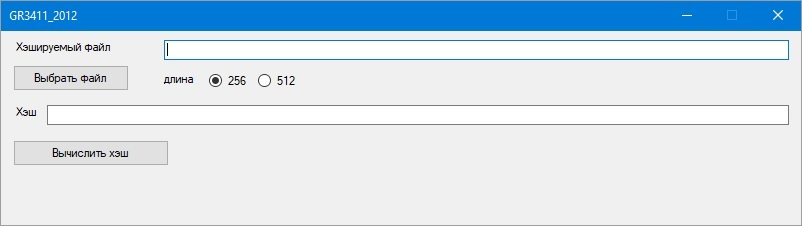
\includegraphics[width=1.0\linewidth]{inc/img/b1}
	\caption{Окно программы для вычисления хэша файлов}
	\label{fig:figB_1}
\end{figure}
\par
В окне, представленном на Рисунке \ref{fig:figB_1}, можно задать имя хэшируемого файла и длину хэша (256 или 512). Для запуска процесса вычисления хэша необходимо нажать кнопку <<Вычислить хэш>>.
\par
Далее представлены результата расчета хэша от некоторых файлов, заданных набором байт. Байты каждого файла и результата расчета хэша представлены $A \in V_{4n}$ и записаны в формате $a_0,\;a_1\,\dots\;,a_{n-1}$, где $a_i\in\mathbb{Z}_{16},\;i=0,\;2,\;\dots,\;n-1$. При этом, $A$ есть $Vec_4(a_0)\|\dots\|Vec_4(a_{n-1})$. Байты исходного файла обозначим как $F$. Значение хэша размера $256$ бит обозначим как $H_{256}$. Значение хэша размера $512$ бит обозначим как $H_{512}$.
{\ttfamily
\par
Пример 1:\\
$F=\;$3031323334353637383930313233343536373839303132333435363738393031323334\\35363738393031323334353637383930313233343536373839303132\\
$H_{256}=\;$9D151EEFD8590B89DAA6BA6CB74AF9275DD051026BB149A452FD84E5E57B5500\\
$H_{512}=\;$1B54D01A4AF5B9D5CC3D86D68D285462B19ABC2475222F35C085122BE4BA1FFA00AD\\30F8767B3A82384C6574F024C311E2A481332B08EF7F41797891C1646F48
\par
Пример 2:\\
$F=\;$D1E520E2E5F2F0E82C20D1F2F0E8E1EEE6E820E2EDF3F6E82C20E2E5FEF2FA20F120EC\\EEF0FF20F1F2F0E5EBE0ECE820EDE020F5F0E0E1F0FBFF20EFEBFAEAFB20C8E3EEF0E5E2FB\\
$H_{256}=\;$9DD2FE4E90409E5DA87F53976D7405B0C0CAC628FC669A741D50063C557E8F50\\
$H_{512}=\;$1E88E62226BFCA6F9994F1F2D51569E0DAF8475A3B0FE61A5300EEE46D961376035F\\E83549ADA2B8620FCD7C496CE5B33F0CB9DDDC2B6460143B03DABAC9FB28
\par
Пример 3:\\
$F=\;$4FEF841A4CD8ED40C398991B0B18CFF540B766FC56A590BA633C47F97ADA4A83943140\\C527AD134A7C3E45DCC9D2BC81D052CC35408B0BAA5EC9B71090F4C5E84D1687D9D809CE92\\A41C80175FB3F19080C528270E1442082695675DF603B988785C8EB24BE2A9C7843991230B\\F34BABD8268FCACB9DDA38D37EB342A2709CA063F79F02243E459E1C61A3D5831FFD334A\\
$H_{256}=\;$02B5722E1375A8E64351E36DE113A131059FAC8E42F33EB48277D6C3B98840BE\\
$H_{512}=\;$DCB9FE9BB8D270771DFF3DAEEBB48D7E86D17600DCEBA5240BC87297D093C1FCC1BE\\DCEFCD79C34EB6A300FE40D9BE366AE3A81A78AFFC070401B8C6D8E7FA86
\par
Пример 4:\\
$F=\;$84D074EEBCDB8255DECC2E6624139CF1C01354488699E0F1AE6AF904B5B48180F7E6EC\\CB2C743BC37FCF60796FB53D9038925EE9DF0135EBEF824052E17DA0294AAE6E3D27D1C54C\\D890C8B7396781F82D69CC235698A0F5B100DCA934E8E2022E362E\\
$H_{256}=\;$D4F3E5DEAB479E26B40FA8ACACFC4E2F509732C1B5AF92D437BD3352E328A56E\\
$H_{512}=\;$AE9E06B039BCE6F640ADA7CB7B18D344C39BBD84F1812B84CF0CC23A58D585123B6A\\E7AE543B1649C9DD548EF45AADA07F5B1E1D08DBA83532DD5D1D7459D747
\par
Пример 5:\\
$F=\;$47FF6967CC12114E397EB18800472578B07CD3B20D788B26F51B17EFADC6880338C0B1\\2DFF6556438651BC334F53A8EDC36A51B2627CB3CE734272B0FA21A172F5AE4F4095F8784B\\25902BBBBC58D7A1732A2C4375D6A0BC0D\\
$H_{256}=\;$49FA7153B608E6E38E6E4F5058E02E598F6912CB70C7B5F07D363643BCB5F93E\\
$H_{512}=\;$44A6329382D6970D77ABD8F49CC11E3CA82E8F845F87684EA18981A9F27E87B729BC\\28174641521E1F4AE200051BD7EA90879553950D1B46D9662ECE59FEB78C
\par
Пример 6:\\
$F=\;$B9BCF3A54965B04A3DA1046857CBF1058CD250F7121A6BD13DCFF55DFC1F0D9232B23E\\BB577F46C60A711B369C0BD361516F49CE6B15D19E512268796F524D1D937235A58C36AD0C\\8B8AECA0FF353432FC940C8DD63E261DE0A06A3517CD56B724FEA2\\
$H_{256}=\;$5D2759000A1F5B46A6CADFF3D04D5F590A475DAB00F5C6BB697D528697CDB67E\\
$H_{512}=\;$8EE49C5B382AA3F48334D95258DEED51BC0BC682243CAAAF1562EA101C888A01FFEA\\F365CCCB16A40CA2445C16C22B1D9A2DF8B4B32DA932F034197CFD0F09FE
\par
Пример 7:\\
$F=\;$D62ED41AC13D43E028309F1BED367DDA46C047554B17C4ECCC78F4BE33357C00930B5C\\CEBFF1CB98FB45F4B0004F47E1507C7163B74DDEBE69E84E494885ADF3B39E87E2DAAF1A55\\F4AE59052214EB7D30136EB7C31849462C9D64D7A2824F7698\\
$H_{256}=\;$5C11C68851E700EB385EA64225E8910972CBBD08E59B98BC0C2B75C7ACFCBCA0\\
$H_{512}=\;$381F13407000C4A931BF3535831826E354D17BBDCFE070A46BC3D71C62393A5A5270\\3B3D9A0F99CE42260F0F89224003D238C45F9AEBF4FE25F9DE4CA82F8CE6
\par
Пример 8:\\
$F=\;$FC62C76507A0611B6F08F3D89B55FDD1183517F52F9B5441B53C4A43B2725EE36C2117\\88B5CB0CCD56A7A9415254020ED9D1691A5FA3D1610D85AFCA551D69FCA90F6B793D751B4C\\29499E87F113EE613A3C6AE1084484C94FB67B301C4177383E\\
$H_{256}=\;$50F4C7486A94E5D881943829D03C4647186C384AB03ED12A200E114CE650AE6B\\
$H_{512}=\;$0CF1E8DB676B4219389D6A033C39327402EB38A45EF9166B901DE6E8889C26E06AD7\\EE8A996EE7777E9FDA65A5201098E3D4C8AD2370CB40DF13F5DC05905FB7
}
\chapter{Код класса цифровой подписи}
\lstinputlisting{inc/src/appendix/V1.cs}
\chapter{Пример работы с цифровой подписью}
Для работы с цифровой подписью в рамках данной работы реализовано 3 приложения. Первое предназначено для задания просмотра и редактирование параметров. Изображение его главного окна представлено на Рисунке \ref{fig:figG_1}.
\begin{figure}[H]
	\centering
	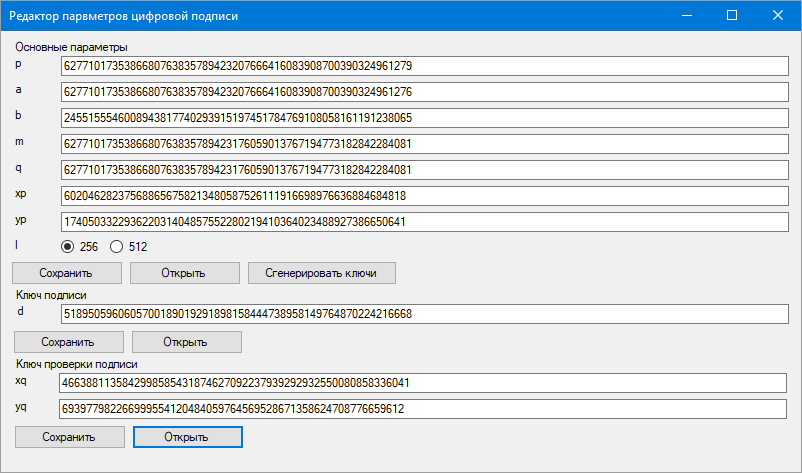
\includegraphics[width=1.0\linewidth]{inc/img/g1}
	\caption{Окно программы для редактирования параметров}
	\label{fig:figG_1}
\end{figure}
\par
В окне программы на Рисунке \ref{fig:figG_1} уже введены данные в десятеричном формате. В дальнейшем будем использовать эти значения. Интерфейс позволяет редактировать и сохранять объекты <<GR3410\_2012\_Parameters>>, <<GR3410\_2012\_SignKey>> и <<GR3410\_2012\_VerifyKey>> в виде XML файлов. Пример кода XML файла показан на Рисунке .
\begin{figure}[H]
	\centering
	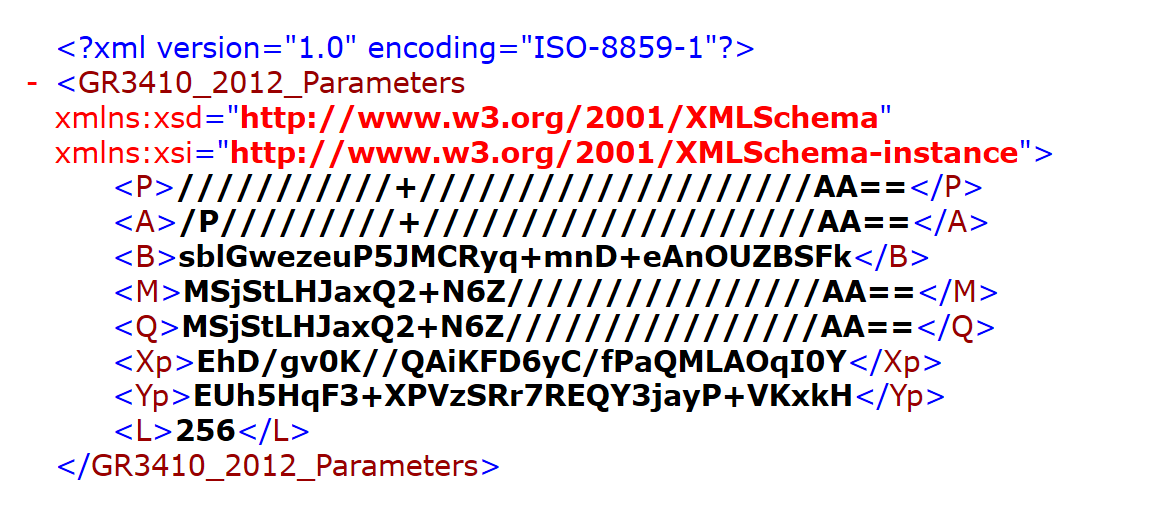
\includegraphics[width=0.9\linewidth]{inc/img/g2}
	\caption{Пример кода XML файла с параметрами}
	\label{fig:figG_2}
\end{figure}
\par
Далее рассмотрим работу приложения для генерации подписи. Изображение главного окна представлено на Рисунке \ref*{fig:figG_3}.
\begin{figure}[H]
	\centering
	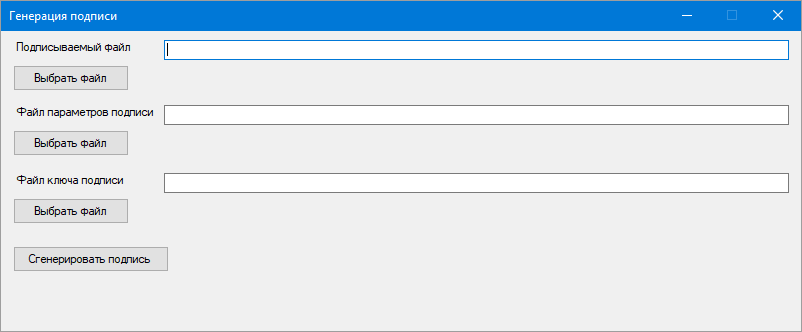
\includegraphics[width=1.0\linewidth]{inc/img/g3}
	\caption{Окно программы для генерации подписи}
	\label{fig:figG_3}
\end{figure}
\par
В окне, изображенном на Рисунке \ref{fig:figG_3}, можно задать подписываемый файл и файлы с параметрами схемы цифровой подписи и ключом подписи. После указания необходимых параметров, для генерации подписи необходимо нажать кнопку <<Сгенерировать подпись>>. Далее начнется расчет хэша. По его завершении, можно сохранить файл, содержащий подпись.
\par
Для примера возьмем файл содержащий следующий набор байт\\
{\ttfamily
$F=\;$D1E520E2E5F2F0E82C20D1F2F0E8E1EEE6E820E2EDF3F6E82C20E2E5FEF2FA20F120EC\\EEF0FF20F1F2F0E5EBE0ECE820EDE020F5F0E0E1F0FBFF20EFEBFAEAFB20C8E3EEF0E5E2FB\\
}
и определенные ранее параметры схемы цифровой подписи и ключ шифрования. Сгенерируем подпись, в результате чего, она будет сохранена в файл (Рисунок \ref{fig:figG_4}). Назовем его <<sign.xml>>.
\begin{figure}[H]
	\centering
	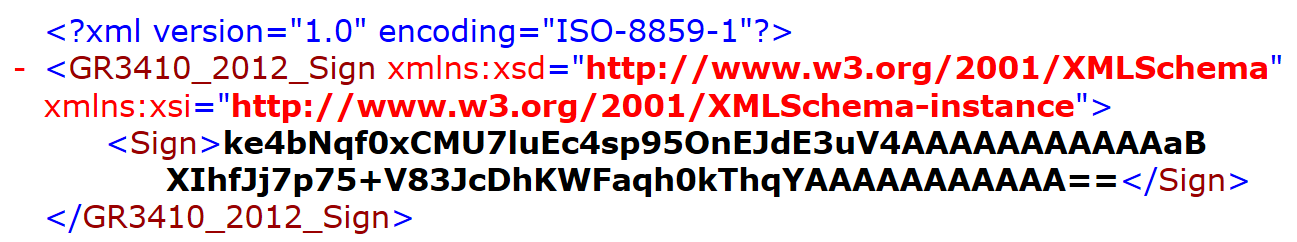
\includegraphics[width=0.9\linewidth]{inc/img/g4}
	\caption{Код файла <<sign.xml>>}
	\label{fig:figG_4}
\end{figure}
\par
Для проверки подписи также используется специальное приложение. Изображение главного окна приложения для проварки подписи показано на Рисунке \ref{fig:figG_5}.
\begin{figure}[H]
	\centering
	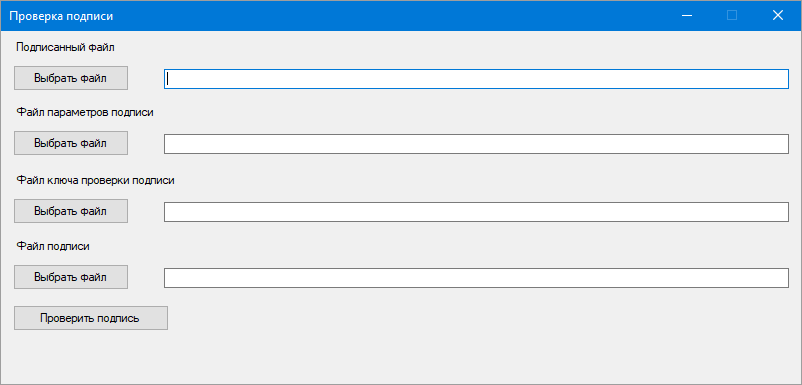
\includegraphics[width=0.9\linewidth]{inc/img/g5}
	\caption{Окно программы для проверки подписи}
	\label{fig:figG_5}
\end{figure}
\par
возьмем тот же файл, те же параметры схемы цифровой подписи и определенный ранее ключ проверки подписи. В качестве подписи зададим файл <<sign.xml>> и запустим процесс проверки подписи. В результате подпись пройдет проверку, о чем мы получим всплывающее сообщение (Рисунок \ref{fig:figG_6}).
\begin{figure}[H]
	\centering
	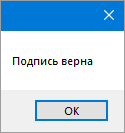
\includegraphics[width=0.2\linewidth]{inc/img/g6}
	\caption{Сообщение о том, что подпись верна}
	\label{fig:figG_6}
\end{figure}
\par
Попробуем изменить подписанный файл. Запишем вместо него следующее\\
{\ttfamily
	$F=\;$01D1E520E2E5F2F0E82C20D1F2F0E8E1EEE6E820E2EDF3F6E82C20E2E5FEF2FA20F120EC\\EEF0FF20F1F2F0E5EBE0ECE820EDE020F5F0E0E1F0FBFF20EFEBFAEAFB20C8E3EEF0E5E2FB.\\
}
При проверке сгенерированной ранее подписи, программа выдаст сообщение о том, что подпись неверна (Рисунок \ref{fig:figG_7}).
\begin{figure}[H]
	\centering
	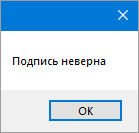
\includegraphics[width=0.23\linewidth]{inc/img/g7}
	\caption{Сообщение о том, что подпись неверна}
	\label{fig:figG_7}
\end{figure}